\documentclass[aspectratio=43]{beamer}
%\usepackage[english]{babel}

%Cargar paquetes
\usepackage[utf8]{inputenc}%Permite usar acentos
\usepackage[spanish]{babel}%Configura el idioma por defecto a español
\usepackage{amsmath}%Introduce términos matemáticos
\usepackage{graphicx}%Permite introducir figuras
\usepackage[options]{natbib}%Bibliografía con estilos %No funcionan estilos en Beamer
\newcommand{\grad}{\hspace{-2mm}$\phantom{a}^{\circ}$}

\usepackage{amsthm}
\usepackage{mathtools}
\usepackage{physics}
\usepackage{calligra}
\usepackage{csquotes}
\usepackage{tensor}
\usepackage[thicklines]{cancel}
\usepackage{tcolorbox}
\usepackage{pstricks}
\usepackage[backend=biber, bibstyle=nature, sorting=nty, citestyle=numeric-comp]{biblatex} %Custom bibliography
    \addbibresource{bib.bib} %Load references


\DeclareMathAlphabet{\mathcalligra}{T1}{calligra}{m}{n}
\DeclareFontShape{T1}{calligra}{m}{n}{<->s*[2.2]callig15}{}
\newcommand{\scriptr}{\mathcalligra{r}\,}
\newcommand{\boldscriptr}{\pmb{\mathcalligra{r}}\,}
\def\rc{\scriptr}
\def\brc{\boldscriptr}
\def\hrc{\hat\brc}
\newcommand{\ie}{\emph{i.e.}} %id est
\newcommand{\eg}{\emph{e.g.}} %exempli gratia
\newcommand{\rtd}[1]{\ensuremath{\left\lfloor #1 \right\rfloor}}
\newcommand{\dirac}[1]{\ensuremath{\delta \left( #1 \right)}}
\newcommand{\diract}[1]{\ensuremath{\delta^3 \left( #1 \right)}}
\newcommand{\e}{\ensuremath{\epsilon_0}}
\newcommand{\m}{\ensuremath{\mu_0}}
\newcommand{\V}{\ensuremath{\mathcal{V}}}
\newcommand{\prnt}[1]{\ensuremath{\left(#1\right)}} %parentheses
\newcommand{\colch}[1]{\ensuremath{\left[#1\right]}} %square brackets
\newcommand{\chave}[1]{\ensuremath{\left\{#1\right\}}}  %curly brackets

\useoutertheme{infolines}
\useinnertheme{rectangles}
\usefonttheme{professionalfonts}


\definecolor{orange}{HTML}{f28165}
\definecolor{gray}{HTML}{303030}
\definecolor{yellow}{HTML}{f0be52}
\definecolor{lightorange}{HTML}{f19e58}

\renewcommand{\CancelColor}{\color{orange}}

\makeatletter
\newcommand{\mybox}[1]{%
  \setbox0=\hbox{#1}%
  \setlength{\@tempdima}{\dimexpr\wd0+13pt}%
  \begin{tcolorbox}[colback=orange,colframe=orange,boxrule=0.5pt,arc=4pt,
      left=6pt,right=6pt,top=6pt,bottom=6pt,boxsep=0pt,width=\@tempdima]
    \textcolor{white}{#1}
  \end{tcolorbox}
}
\makeatother

\usecolortheme[named=orange]{structure}
\usecolortheme{sidebartab}
\usecolortheme{orchid}
\usecolortheme{whale}
\setbeamercolor{alerted text}{fg=yellow}
\setbeamercolor{block title alerted}{bg=alerted text.fg!90!black}
\setbeamercolor{block title example}{bg=lightorange!60!black}
\setbeamercolor{background canvas}{bg=gray}
\setbeamercolor{normal text}{bg=gray,fg=white}

\setbeamertemplate{footline}
        {
      \leavevmode%
      \hbox{%
      \begin{beamercolorbox}[wd=.333333\paperwidth,ht=2.25ex,dp=1ex,center]{author in head/foot}%
        \usebeamerfont{author in head/foot}\insertshortauthor~~(\insertshortinstitute)
      \end{beamercolorbox}%
      \begin{beamercolorbox}[wd=.333333\paperwidth,ht=2.25ex,dp=1ex,center]{title in head/foot}%
        \usebeamerfont{title in head/foot}\insertshorttitle
      \end{beamercolorbox}%
      \begin{beamercolorbox}[wd=.333333\paperwidth,ht=2.25ex,dp=1ex,center]{date in head/foot}%
        \usebeamerfont{page number in head/foot}\insertframenumber/\inserttotalframenumber%\hspace*{2em}

    %#turning the next line into a comment, erases the frame numbers
        %\insertframenumber{} / \inserttotalframenumber\hspace*{2ex} 

      \end{beamercolorbox}}%
      \vskip0pt%
    }


\setbeamertemplate{blocks}[rectangle]
\setbeamercovered{dynamic}

\setbeamertemplate{section page}
{
	\begin{centering}
		\begin{beamercolorbox}[sep=27pt,center]{part title}
			\usebeamerfont{section title}\insertsection\par
			\usebeamerfont{subsection title}\insertsubsection\par
		\end{beamercolorbox}
	\end{centering}
}

%\setbeamertemplate{subsection page}
%{
%	\begin{centering}
%		\begin{beamercolorbox}[sep=12pt,center]{part title}
%			\usebeamerfont{subsection title}\insertsubsection\par
%		\end{beamercolorbox}
%	\end{centering}
%}

\newcommand{\hlight}[1]{\colorbox{violet!50}{#1}}
\newcommand{\hlighta}[1]{\colorbox{red!50}{#1}}
\title{Metodología de un proyecto de simulación} %->->->->-> Check hyperref title <-<-<-<-<-
%\subtitle{And Some Things About It}
\author[C.J. Uribe-Martes]{Carlos Javier Uribe Martes}
\institute[CUC]{
    Ingeniería Industrial%
    \\%
    Universidad de la Costa%
} %You can change the Institution if you are from somewhere else
\date{Febrero 8, 2020}
%\logo{\includegraphics[width= 0.2\textwidth]{images/a-logo.png}}

\begin{document}
    
    \frame{\titlepage}
    
    \begin{frame}{Contenido}
        \tableofcontents
    \end{frame}
    
    \section{Pasos en un proyecto de simulación}

\frame{\sectionpage}

\begin{frame}{Pasos en un proyecto de simulación}
    \begin{itemize}
        \item Hay un conjunto de pasos básicos para la realización de un proyecto de simulación.
        \item Tenga en cuenta que NO es un proceso secuencial.
        \item En ocasiones será necesario agregar o suprimir algunos pasos.
    \end{itemize}
\end{frame}

\begin{frame}{Metodología adaptada de \cite{BCN} and \cite{LK}}
    \begin{figure}
        \centering
        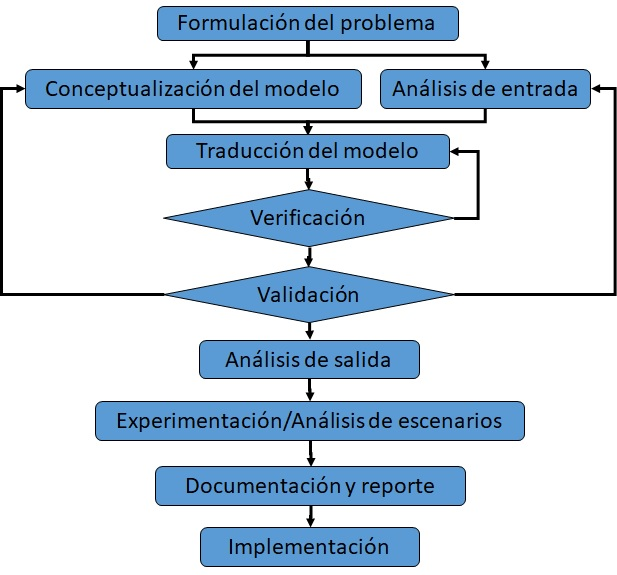
\includegraphics[width=7.5cm]{images/Metodologia.jpg}
        %\caption{Adaptado de \cite{BCN} and \cite{LK}}
        \label{fig:metodología}
    \end{figure}
\end{frame}

\begin{frame}{Formulación del problema}
    \begin{itemize}
        \item El estudio comienza con una declaración del problema.
        \item Se determinan los objetivos y el alcance del proyecto, se identifica al tomador de decisiones, al usuario y al modelista.
        \item Los objetivos indican las preguntas que serán respondidas.
    \end{itemize}
\end{frame}

\begin{frame}{Conceptualización del modelo}
    \begin{itemize}
        \item Se basa en la capacidad de abstraer los elementos esenciales del problema y sus interacciones.
        \item Emplea supuestos para caracterizar el sistema de forma básica y enriquecer el modelo hasta encontrar una aproximación útil.
    \end{itemize}
\end{frame}

\begin{frame}{Recolección de datos y análisis de entrada}
    \begin{itemize}
        \item Identificación, recolección y análisis de los datos necesarios para el estudio.
        \item Incluya datos del desempeño del sistema para validación.
    \end{itemize}
\end{frame}

\begin{frame}{Traducción del modelo}
    \begin{itemize}
        \item Se generan las instrucciones necesarias para lograr que el modelo pueda ser ejecutado en una computadora.
        \item Se debe decidir entre un lenguaje de programación general o un lenguaje de propósito específico.
    \end{itemize}
\end{frame}

\begin{frame}{Análisis de salida}
    \begin{itemize}
        \item Estimación de las medidas de desempeño del sistema y los diseños que están siendo simulados. 
        \item Se especifican los parámetros de corrida:
        \begin{enumerate}
            \item Número de réplicas independientes.
            \item Longitud de corrida.
            \item Longitud del periodo de calentamiento.
        \end{enumerate}
    \end{itemize}
\end{frame}

\begin{frame}{Experimentación y Análisis de escenarios}
    \begin{itemize}
        \item Determina las alternativas a evaluar con la simulación.
        \item Se comparan las alternativas en términos de las medidas de desempeño y costos.
    \end{itemize}
\end{frame}

\begin{frame}{Documentación y reporte}
    \begin{itemize}
        \item Reportar de forma clara y concisa en un documento:
        \begin{enumerate}
            \item Supuestos empleados.
            \item Análisis de resultados.
            \item Animación para comunicar los detalles del modelo.
            \item Discusión de la construcción del modelo y validación.
        \end{enumerate}
    \end{itemize}
\end{frame}

    \section{Verificación y validación}

\frame{\sectionpage}

\begin{frame}{Verificación y validación}
    %\begin{itemize}
        %\item La verificación y la validación se ocupan de determinar si un modelo y sus resultados son 'correctos' para un uso o propósito específico.
        \begin{itemize}
            \item La \textit{verificación} se define como 'asegurar que el modelo programado y su implementación sean correctos'.
            \item La \textit{validación} se define como la 'comprobación de que el modelo de simulación dentro de su dominio de aplicabilidad posee un rango satisfactorio de precisión consistente con la aplicación prevista del modelo'.
        \end{itemize}
    %\end{itemize}    
\end{frame}

\begin{frame}{Proceso de desarrollo de modelos}
    \begin{figure}
        \centering
        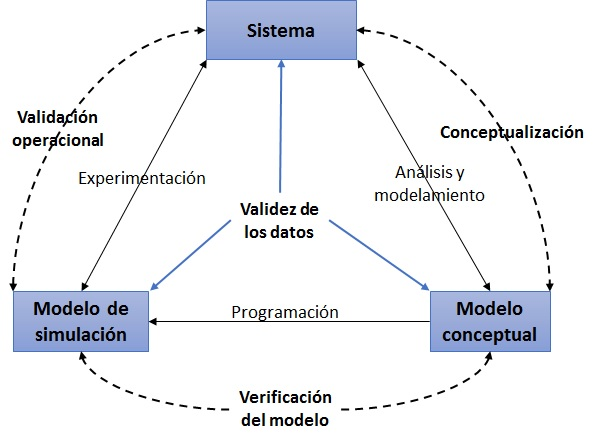
\includegraphics[width=9cm]{images/vandv.jpg}
        %\caption{Proceso de desarrollo de modelos}
        \label{fig:my_label4}
    \end{figure}
\end{frame}

\begin{frame}{Verificación}
    \begin{itemize}
        \item La verificación evalúa la exactitud de la representación formal del modelo previsto, a través de:
        \begin{enumerate}
            \item Depurador
            \item Animación
            \item Estadísticas básicas de las corridas de prueba
            \item Modelos de teoría de colas
        \end{enumerate}
    \end{itemize}
\end{frame}

\begin{frame}{Validación}
    \begin{itemize}
        \item La validación compara (estadísticamente) las medidas de desempeño del modelo, obtenidas en las corridas de prueba, con sus contrapartes en el sistema.
    \end{itemize}
\end{frame}

\begin{frame}{Validación - Ejemplo}
    \begin{itemize}
        \item Se tiene una muestra de demoras diarias en un cierto proceso del sistema real y la serie de datos de dichas demoras en el modelo simulado.
        \item Se podría definir una muestra de las diferencias observadas como \begin{equation*}
            G_i=\Hat{D_i}-\bar{D_i},~i=1,\dots, N
        \end{equation*}
        que sigue una distribución normalmente distribuida con media $\mu_G$ y varianza $\sigma^2_G$. Donde $\bar{D_i}$ es la media observada de la demora para el día $i$ en el sistema real y $\Hat{D_i}$ es la media estimada de la demora en el día $i$ tomada del modelo de simulación, para los días $i=1,\dots, N$.
    \end{itemize}
\end{frame}

\begin{frame}{Validación - Ejemplo}
    \begin{itemize}
        \item Se plantean las hipótesis 
        \begin{eqnarray*}
            H_0:~\mu_G=0\\
            H_1:~\mu_G \neq 0
        \end{eqnarray*}
        \item Bajo la hipótesis nula, el estadístico
        \begin{equation*}
            t_{N-1}=\frac{\bar{G}-\mu_G}{\frac{S_G}{\sqrt{N}}}
        \end{equation*}
        se distribuye de acuedo a un distribución $t$ de Student, con $N-1$ grados de libertad, donde $\bar{G}$ y $S_G$ son la media y desviación estándar de la muestra $\{G_1,\dots,G_N\}$, respectivamente.
    \end{itemize}
\end{frame}

\begin{frame}{Validación - Ejemplo}
    \begin{itemize}
        \item Para un nivel de significancia $\alpha$, el correspondiente intervalo de confianza es
        \begin{equation*}
            \bar{G}-t_{\frac{\alpha}{2},N-1}\frac{S_G}{\sqrt{N}}\leq \mu_G \leq \bar{G}+t_{\frac{\alpha}{2},N-1}\frac{S_G}{\sqrt{N}}
        \end{equation*}
        \item Si el intervalo de confianza anterior contiene 0, no se puede rechazar $H_0$ en el nivel de significancia $\alpha$, lo que indica que la prueba respalda la validez del modelo.
    \end{itemize}
\end{frame}

    \section{Implementación}

\frame{\sectionpage}

\begin{frame}{Implementación}
    \begin{itemize}
        \item Implica colocar en práctica las decisiones tomadas con base en el estudio.
        \item La credibilidad y la usabilidad se ven realzadas cuando el usuario y el tomador de decisiones participan activamente en todo el proceso.
        \item La animación puede ser clave para visualizar las ventajas de la implementación.
    \end{itemize}
\end{frame}


\begin{frame}{Credibilidad y usabilidad}
    \begin{itemize}
        \item La \textit{credibilidad} del modelo tiene que ver con desarrollar en el usuario y el tomador de decisiones la confianza para usar el modelo y la información derivada del mismo.
        \item La \textit{usabilidad} del modelo determina que el modelo y sus instrucciones para el usuario son fáciles de usar.
    \end{itemize}    
\end{frame}

    \section*{Referencias} %You can remove this if you do not want to use it
        \begin{frame}{Referencias}
            \printbibliography
        \end{frame}
     
    \section{}   
        \begin{frame}{}
            \begin{figure}
                \centering
                
\includegraphics[width=6cm]{images/model.png}
                %\caption{Caption}
                %\label{fig:my_label}
            \end{figure}
        \end{frame}
      
\end{document}